\cleardoublepage

\section{记号}
\begin{enumerate}
      \item 设$b$是大于等于$2$的正整数,记$x\in[0,1]$以$b$为基数的展开形式为$x=0.x_1x_2\cdots x_n\cdots$,其中$x_i\in\{0,1,\cdots,b-1\}$,也就是说$x=\underset{i=1}{\overset{\infty}{\sum}}x_ib^{-i}$。
\end{enumerate}



\section{于汉的研究}

于汉在他的文章《Weak tangent and level set of the Takagi function》一文中介绍了Takagi函数,并证明了在特定参数下Takagi函数的一些性质。

\begin{definition}[Takagi 函数]
        以下函数称为Takagi函数
        $$
            T_{a,b}(x)=\sum_{n=0}^\infty a^nT(b^nx),
        $$
        其中,$a<1,b>1,ab\ge1$,且$T:\mathbb{R}\rightarrow\mathbb{R}$是周期为$1$ 的帐篷函数,其在区间$[0,1]$上的定义为,
        $$
            T(x)=
            \begin{cases}
                x~~~~~~,x\in[0,\frac{1}{2}],\\
                1-x,x\in[\frac{1}{2},1].
            \end{cases}
        $$

        \begin{definition}[Littlewood多项式]
            称所有系数的取值都在$\{1,-1\}$中的$k$阶多项式为$k$阶Littlewood多项式,即,
            $$
                \sum_{n=0}^k\epsilon_nx^n=0,
            $$
            其中,$\epsilon_n\in\{1,-1\}$。
        \end{definition}
\end{definition}

\subsection{Takagi函数的水平集及其Hausdorff维数}

\begin{definition}[水平集]
    设函数$f:[0,1]\rightarrow\mathbb{R}$,$\forall y \in\mathbb{R}$,定义函数$f$的水平集为,
    $$
        L(y)=\{x\in[0,1]:f(x)=y\}\times\{y\}.
    $$
\end{definition}

于汉的第一个结论为,参数$a,b$满足$0<a<1,b>1,2|b,ab\ge1,ab$为$k-1$阶Littlewood多项式的根的Takagi函数具有一个较大的水平集,这个水平集的Hausdorff维数不小于$\frac{1}{k}$。

\begin{proof}
    由条件,$\exists\epsilon_n\in\{1,-1\},n=0,1,\cdots,k-1$,使得$ab$为以下$k-1$阶Littlewood多项式的根,
    $$
        \sum_{n=0}^{k-1}\epsilon_n(ab)^n=0.
    $$

    取$T_{a,b}(x)$的前$k$项部分和,记为$F_1(x)$,
    $$
        F_1(x)=\sum_{n=0}^{k-1}a^nT(b^nx),
    $$
    显然,对任意的正整数$m$,$x=mb^{-k}$为$F_1(x)$的不可导点。

    我们有
    $$
        \begin{aligned}
            F_1(1-x) & =\sum_{n=0}^{k-1}a^nT(b^n(1-x))=\sum_{n=0}^{k-1}a^nT(b^n-b^nx) \\
                   & =\sum_{n=0}^{k-1}a^nT(1-b^nx)=\sum_{n=0}^{k-1}a^nT(b^nx)=F_1(x).
        \end{aligned}
    $$
    故$F_1(x)$关于直线$x=\frac{1}{2}$对称。

    对$F_1(x)$求导,可得
    $$
        F_1'(x)=\sum_{n=0}^{k-1}(ab)^nT'(b^nx).
    $$

    我们记$\epsilon_n(x)=T'(b^nx)$,则
    $$
        F_1'(x)=\sum_{n=0}^{k-1}\epsilon_n(x)(ab)^n,
    $$
    其中,$\epsilon_n(x)\in\{1,-1\}$,其取值取决于$x$以$b$为基数的展开式。若$x$以$b$为基数的展开式为
    $$
        x=0.x_1x_2\cdots
    $$
    由于$T(x)$周期为$1$,其导数的周期也为$1$,故有
    $$
        T'(b^nx)=T'(x_1x_2\cdots x_n.x_{n+1}\cdots x_k\cdots)=T'(0.x_{n+1}\cdots x_k\cdots),n=0,1,\cdots,k-1.
    $$
    则有
    $$
        \epsilon_n(x)=
        \begin{cases}
            1,x_{n+1}\in[0,\frac{b}{2}),\\
            -1,x_{n+1}\in[\frac{b}{2},b),
        \end{cases},n=0,1,\cdots,k-1.
    $$

    因此,我们可以找到$b_1,b_2,\cdots,b_k$并令$x_i=b^1_i,i=1,2,\cdots,k$,即可使$\epsilon_n(x)=\epsilon_n,n=0,1,\cdots,k-1$,从而有
    $$
        F_1'(x)=\sum_{n=0}^{k-1}\epsilon_n(x)(ab)^n=\sum_{n=0}^{k-1}\epsilon_n(ab)^n=0.
    $$
    此时,我们仅改变$b_k$的取值,若$b_k<\frac{b}{2}$,则令其取遍$[0,\frac{b}{2})$,反之则取遍$[\frac{b}{2},b)$,则我们得到了$\frac{b}{2}$个长度为$\frac{1}{b^k}$的区间,其为被仅挖去了点$x=mb^{-k}$的连续区间,故在这些区间上,我们得到$F_1'(x)=0$,存在$a_1\in\mathbb{R}$,使得$F_1(x)=a_1$。

    因为$\underset{n=0}{\overset{k-1}{\sum}}\epsilon_n(ab)^n=0$,则有$\underset{n=0}{\overset{k-1}{\sum}}(-\epsilon_n)(ab)^n=0$。
    又因为$F_1(x)$关于直线$x=\frac{1}{2}$对称,故我们可以找到与上述$\frac{b}{2}$个区间一一对称的$\frac{b}{2}$个区间,在这些区间上$\epsilon_n(x)=-\epsilon_n$,且有$F_1(x)=a_1$。

    至此,我们找到了$b$个长度为$\frac{1}{b^k}$的区间,由此,我们可以得到一个$F_1(x)$的水平集。

    取Takagi函数的第二个$k$项部分和,记为$F_2(x)$
    $$
        F_2(x)=\sum_{n=k}^{2k-1}a^nT(b^nx)=\sum_{n=0}^{k-1}a^k\cdot a^nT(b^n\cdot b^kx)=a^kF_1(b^kx).
    $$
    不难看出,存在$b_{k+1},b_{k+2},\cdots,b_{2k}$并令$x_i=b_i,i=k+1,\cdots,2k$,即可使$F_2'(x)=(ab)^kF_1'(b^kx)=0$,即存在$a_2\in\mathbb{R}$,使得$F_2(x)=a_2$。

    同上,我们令$b_{2k}$取遍它所在的一半区间,并加上与这些区间对称的区间。再将前$k$个$x_i$的取值继承下来,这样,我们就得到了$b^2$个长度为$\frac{1}{b^{2k}}$的区间,这可以构成$F_1(x)+F_2(x)$的一个水平集。

    不断重复上述过程,不难得到,在第$m$次迭代时,我们可以构造出以下区间
    $$
        L_m=\{x:x=0.b_1b_2\cdots b_kb_{k+1}\cdots b_{2k}\cdots b_{(m-1)k+1}\cdots b_{mk}x_{mk+1}\cdots\}
    $$
    使得$\forall x\in L_m$,有$T'(b^nx)=\epsilon_{N(n)}$,或$T'(b^nx)=-\epsilon_{N(n)},n=1,2,\cdots,mk$其中,$N(n)=n(\mathrm{mod}~b)$。

    这样,我们得到了$b^m$个长度为$\frac{1}{b^mk}$的区间,在这些区间上,$\exists y_m\in\mathrm{R}$,使得,$\underset{n=1}{\overset{m}{\sum}}F_n(x)=y_m$由此,我们可以构造水平集$L_m(y_m)$

    $$
        L_m(y_m)=\{(x,y_m):x\in L_m\}.
    $$


\end{proof}

\subsection{Takagi函数图像的Assouad维数}


\section{类Takagi函数的结论}

\begin{enumerate}

      \item 对区间$I$,我们用$|I|$表示区间的长度。
      \item 给定区间族$\mathbb{I}=\{I_1,I_2,\cdots,I_N\}$,若$\forall i,j,\frac{|I_i|}{|I_j|}\in\mathbb{Q}$,则定义
      $$
            \gcd(\mathbb{I})=\sup\big\{T:\frac{|I_i|}{T}\in\mathbb{Z},i=1,2,\cdots,N\big\}.
      $$
      \item 对区间族$\mathbb{I}$中的区间$I_i$,我们定义
      $$
            n(I_i)=\frac{|I_i|}{gcd(\mathbb{I})},i=1,2,\cdots,N.
      $$
      显然,对任意的$1\le i\le N,n(I_i)\in\mathbb{Z}$。
      \item 我们定义
      $$
            n(\mathbb{I})=\sum_{i=1}^Nn(I_i).
      $$
      不难得
      $$
            |I_i|=\frac{n(I_i)}{n(\mathbb{I})}\sum_{j=1}^N|I_j|.
      $$
      \item 对定义在$[0,1]$上的实值函数$f(x)$,我们定义其水平集为$L(y)=\{x\in[0,1]:f(x)=y,y\in\mathbb{R}\}$。
      \item $\lfloor x \rfloor$表示不超过$x$的最大整数。
      \item $\forall a\in\mathbb{R}^2,R\in\mathbb{R},S(a,R)$表示以$a$为中心,边长为$2R$的正方形。
      \item $\forall a\in\mathbb{R}^2,R\in\mathbb{R},B(a,R)$表示以$a$为球心,半径为$R$的球。
      \item $\Gamma_T$表示函数$T(x)$的图像,即$\Gamma_T=\{(x,y):y=T(x),x\in\mathbb{R}\}$。
      \item 对集合$F$,$N_r(F)$表示以半径为$r$的球对$F$进行覆盖所需的最小覆盖数。
      \item 对集合$F$,我记以下为其相邻正方形覆盖数
      $$
            N(F\cap S(a,R),r)=\Big|\{(i,j)\in\mathbb{Z}^2\cap[0,\lfloor\frac{R}{r}\rfloor]^2:\\
                  S((a-\frac{R}{2}+\frac{r}{2}+ir,a-\frac{R}{2}+\frac{r}{2}+jr),r)\cap F\neq\emptyset\}\Big|.
      $$
      由于$\exists C>0$,使得$C^{-1}N_r(F\cap B(a,R))\le N(F\cap S(a,R),r)\le CN_r(F\cap B(a,R))$,在本文中我们用更方便的相邻正方形覆盖数替代球覆盖数。
\end{enumerate}

\section{预备知识}
\subsection{可分割折线函数}

设$h(x)$是周期为1,且关于直线$x=\frac{1}{2}$对称,并且在$[0,1]$区间上为分段线性的连续函数,即$\exists0=x_0<x_1<\cdots<x_N=1$,使得$\forall 1\le i\le N$,$h(x)$在$[x_{i-1},x_i]$上为线性函数。

同时,根据$h(x)$的不可导点对$[0,1]$区间进行划分,可以得到$\mathbb{I}=\{I_1,I_2,\cdots,I_N\}$,其中$I_1,\cdots,I_N$从左到右排列。

若$N\ge2,\forall i,j\in\{1,2,\cdots,N\},\frac{|I_i|}{|I_j|}\in\mathbb{Q}$,则称$h(x)$为可分割折线函数。

\subsection{Littlewood多项式}
若一个$n$阶多项式的所有系数都在$\{1,-1\}$中取值,则称该多项式为一个$n$阶的Littlewood多项式。

\subsection{维数定义}
\subsubsection{盒维数}
对集合$F$,其的盒维数为
$$
      \mathrm{\dim_B}F=-\frac{\log N_r(F)}{\log r}.
$$

\subsubsection{Hausdorff维数}
对集合$F$,其Hausdorff维数为
$$
      \mathrm{\dim_H}F=\inf\{s:\forall\delta>0,\exists\{U_i\}_{i=1}^\infty,\mbox{使得}\bigcup_{i=1}^\infty U_i\supset F,\mbox{且}\sum_{i=1}^\infty (\mathrm{diam}~U_i)^s<\delta\}.
$$

\subsubsection{Assouad维数}
对集合$F$,其Assouad维数为
$$
      \mathrm{\dim_A}F=\inf\{s:(\exists C>0)(\forall R>0)(\forall r\in(0,R))(\forall x\in F),N_r(B(x,R)\cap F)\le C\Big(\frac{R}{r}\Big)^s\}.
$$

\section{结论}

\subsection{结论1——大型水平集}

假设$h(x)$为可分割函数,其在$[0,1]$上按不可导点被分割的区间族为$\mathbb{I}=\{I_1,I_2,\cdots,I_N\}$,其中$I_1,\cdots,I_N$从左到右排列。并设$h(x)$在区间$I_i$上的导数值为$K_i$。设$\mathbb{I}$中$h(x)$的导数不为$0$的区间中,区间长度最大的为$I_{J^*}$,记其上的导数为$K_{J^*}$,由于$h(x)$关于$x=\frac{1}{2}$对称,故$|I_{N+1-J^*}|=|I_{J^*}|$且$I_{N+1-J^*} $上的导数为$-K_{J^*}$。

我们定义类Takagi函数$H_{a,b}(x)$
$$
      H_{a,b}(x)=\sum_{n=0}^\infty a^nh(b^nx).
$$

其中$a,b$满足$0<a<1,b>1$,$ab$为$k-1$阶Littlewood多项式的根,且$n(\mathbb{I})|b$,则对函数$H_{a,b}(x)$,有
$$
      \exists y\in\mathbb{R},\mathrm{dim_H}L(y)\ge\frac{1}{k}\Big(1+\log_b2|I_{J^*}|\Big).
$$

\begin{proof}
由条件,$\exists \epsilon_n\in\{1,-1\},n=0,1,\cdots,k-1$,使得$ab$为以下$k-1$阶Littlewood多项式的根
$$
      \sum_{n=0}^{k-1}\epsilon_n(ab)^n=0.
$$
我们取$H_{a,b}(x)$的前$k$项部分和,记为$H_1(x)$,
$$
      H_1(x)=\sum_{n=0}^{k-1}a^nh(b^nx),
$$
我们有
$$
    \begin{aligned}
        H_1(1-x)&=\sum_{n=0}^{k-1}a^nh(b^n(1-x))\\
                &=\sum_{n=0}^{k-1}a^nh(b^n-b^nx)\\
                &=\sum_{n=0}^{k-1}a^nh(1-b^nx)\\
                &=\sum_{n=0}^{k-1}a^nh(b^nx)=H_1(x).
    \end{aligned}
$$
故$H_1(x)$关于直线$x=\frac{1}{2}$对称。

对其求导,可得
$$
      H_1'(x)=\sum_{n=0}^{k-1}(ab)^nh'(b^nx),
$$
我们记$\epsilon_n(x)=h'(b^nx)$,则
$$
      H_1'(x)=\sum_{n=0}^{k-1}\epsilon_n(x)(ab)^n,
$$
若我们可令$\epsilon_n(x)=\epsilon_n$,我们可得$H_1'(x)=0$。

$\forall x\in[0,1]$将$x$以$b$为基数展开,并假设其展开形式为$x=0.x_1x_2\cdots x_n\cdots$。

$\forall b_1,b_2,\cdots,b_k\in\{0,1,2\cdots,b-1\}$,定义
$$
      I^1(b_1b_2\cdots b_k)=\{x:x\mbox{展开式小数点后的第}1\mbox{项到第}k\mbox{项为}b_1b_2\cdots b_k\}.
$$

根据$b_n,n=1,2,\cdots,k$的取值,我们一共可以生成$b^k$个连续的,长度为$\frac{1}{b^k}$的上述区间。由于$n(\mathbb{I})|b$,故有$\frac{|I_i|}{1/b^k}=|I_i|\cdot b^k=\frac{n(I_i)}{n(\mathbb{I})}\cdot b^k\in\mathbb{Z},i=1,2,\cdots,N$。

我们知道,对$x\in I^1(b_1b_2\cdots b_k)$,有
$$
      x=0.b_1b_2\cdots b_kx_{k+1}x_{k+2}\cdots,
$$
$$
b^{n}x=b_1b_2\cdots b_{n}.b_{n+1}\cdots b_kx_{k+1}x_{k+2}\cdots,0\le n\le k-1.
$$

又有$h(x)$的周期为1,则其导数的周期也为1。故$\forall0\le n\le k-1$,
$$
      h'(b^nx)=h'(b_1b_2\cdots b_n.b_{n+1}\cdots b_kx_{k+1}\cdots)=h'(0.b_{n+1}\cdots b_kx_{k+1}\cdots).
$$

因此,我们可得以下结论:

$$
      \epsilon_n(x)=h'(b^nx)=h'(0.b_{n+1}\cdots b_k\cdots)=            K_j,b_{n+1}\in{[}\frac{b}{n(\mathbb{I})}\sum_{i=1}^{j-1}n(I_i),\frac{b}{n(\mathbb{I})}\sum_{i=1}^{j}n(I_i){)},j=1,2,\cdots,N.
$$

由此,我们可以找到对应的$\tilde{b}_1,\tilde{b}_2,\cdots,\tilde{b}_{k-1},\tilde{b}_k$,使得$\forall x\in I^1(\tilde{b}_1\tilde{b}_2\cdots \tilde{b}_k),\epsilon_n(x)=\epsilon_nK_{J^*},n=0,1,2,\cdots,k-1$。若给定$\tilde{b}_1,\tilde{b}_2,\cdots,\tilde{b}_{k-1}$,我们可以令$\tilde{b}_k$取遍${[}\frac{b}{n(\mathbb{I})}\sum_{i=0}^{J^*-1}n(I_i),\frac{b}{n(\mathbb{I})}\sum_{i=0}^{J^*}n(I_i){)}$
或${[}\frac{b}{n(\mathbb{I})}\sum_{i=0}^{N-J^*}n(I_i),\frac{b}{n(\mathbb{I})}\sum_{i=0}^{N+1-J^*}n(I_i){)}$,这样,我们得到了$\frac{n(I_{J^*})}{n(\mathbb{I})}b$个长度为$\frac{1}{b^k}$的区间,这些区间相互连接,仅被挖去了端点。同时,在这些区间上,我们有
$$
      H_1'(x)=\sum_{n=0}^{k-1}\epsilon_n(x)(ab)^n=\sum_{n=0}^{k-1}\epsilon_nK_{J^*}(ab)^n=K_{J^*}\sum_{n=0}^{k-1}\epsilon_n(ab)^n=0.
$$
故在这些区间上$H_1(x)$取常值,记为$y_1$。

由于$\underset{n=0}{\overset{k-1}{\sum}}\epsilon_n(ab)^n=0$,所以$\underset{n=0}{\overset{k-1}{\sum}}(-\epsilon_n)(ab)^n=0$。

由于$H_1(x)$关于$x=\frac{1}{2}$对称,我们可以找到另外的$\frac{n(I_J^*)}{n(\mathbb{I})}b$个区间,在这些区间上,$\epsilon_n(x)=-\epsilon_nK_M$,故$H'_1(x)=0,H_1(x)\equiv y_1$。由此,我们找到了$H_1(x)$的$y_1$的一个水平集,它由$\frac{2n(I_J^*)}{n(\mathbb{I})}$个长度为$\frac{1}{b^k}$的区间构成,我们将这个水平集记为$L_1$。

现取第二个$k$项部分和,记为$H_2(x)$
$$
      \begin{aligned}
            H_2(x)&= \sum_{n=k}^{2k-1}a^nh(b^nx)\\
                  &= \sum_{n=0}^{k-1}a^{k+n}h(b^{k+n}x)\\
                  &= a^kH_1(b^kx).
      \end{aligned}
$$

因此,我们可以构造如下区间:
$$
      I^2(b_{k+1}b_{b+2}\cdots b_{2k})=\{x:x\mbox{展开式小数点后的第}k+1\mbox{项到第}2k\mbox{项为}b_{k+1}b_{k+1}\cdots b_{2k}\}.
$$

考虑$I^1\cap I^2$,这是将原先长为$\frac{1}{b^k}$的区间再进行$b^k$等分,即分成长为$\frac{1}{b^{2k}}$的区间。

现对$b_{k+1}\cdots b_{2k}$按与上述相同的取法,这样可以在第一轮选出的$\frac{2n(I_J^*)}{n(\mathbb{I})}b$个区间内,每个区间内可以再找出$\frac{2n(I_J^*)}{n(\mathbb{I})}b$个小区间。故共可得$[\frac{2n(I_J^*)}{n(\mathbb{I})}b]^2$个长度为$\frac{1}{b^{2k}}$的区间,在这些区间上,同时满足$H'_1(x)=0,H'_2(x)=0$,且由于周期性与对称性,在这些区间上,$H_1(x)$取常值$y_1,H_2(x)$取常值,记为$y_2$,并将此水平集记为$L_2$。

按此方法迭代,我们可以在第$m$次迭代时,我们可得$[\frac{2n(I_J^*)}{n(\mathbb{I})}b]^m$个长度为$\frac{1}{b^{mk}}$的区间构成的一个$\sum_{t=1}^mH_t(x)$的水平集,我们将这个水平集记为$L_m$,对这个集合进行Hausdorff维数的计算时,我们可以取$[\frac{2n(I_J^*)}{n(\mathbb{I})}b]^m$个直径为$\frac{1}{b^{mk}}$的小集合,这样的集合恰好可以覆盖$L_m$。

由此,我们可以得出结论,$H_{a,b}(x)=\sum_{n=0}^\infty a^nh(b^nx)$具有一个水平集$L=\cap_{t=1}^\infty L_t$,其中$y=\sum_{t=1}^\infty y_t$。

则$\forall \delta>0$,其Hausdorff维数$s$有:

$$
      \lim_{m\rightarrow\infty}\Big[\frac{2n(I_J^*)}{n(\mathbb{I})}b\Big]^m*\Big[\frac{1}{b^{mk}}\Big]^s<\delta.
$$

即,
$$
      \lim_{m\rightarrow\infty}\Big[\frac{2n(I_J^*)}{n(\mathbb{I})}b*\frac{1}{b^{ks}}\Big]^m<\delta.
$$

即,
$$
      \frac{2n(I_J^*)}{n(\mathbb{I})}b^{1-ks}<1.
$$

从而有:
$$
      1-ks<\log_b\frac{n(\mathbb{I})}{2n(I_J^*)}.
$$

又有,$\frac{n(I_J^*)}{n(\mathbb{I})}=|I_J^*|$,我们可得,
$$
      s>\frac{1}{k}\Big(1-\log_b\frac{n(\mathbb{I})}{2n(I_J^*)}\Big)=\frac{1}{k}\Big(1+\log_b2|I_J^*|\Big).
$$

\end{proof}

\subsection{结论2——函数图像的Assouad维数}

\begin{lemma}
      若$1<\beta<2$,则有,$\forall k\in\mathbb{Z}^+$,存在一个序列$\{\epsilon_n\}_{n=0}^k\in\{-1,1\}$,使得,
      $$
            |\sum_{n=0}^k\epsilon_n\beta^n|<\frac{1}{\beta-1}.
      $$
\end{lemma}

\begin{proof}
      我们构造$f_1(x)=\beta x+1,f_{-1}(x)=\beta x -1$,则我们可得:
      $$
            \sum_{n=0}^k\epsilon_n\beta^n=\epsilon_0+\beta(\epsilon_1+\beta(\cdots+\beta(\epsilon_k+\beta*0)))=f_{\epsilon_0}\circ f_{\epsilon_1}\circ \cdots f_{\epsilon_k}(0).
      $$
      此时,我们可以绘制以下图像,
      \begin{figure*}[htbp]
            \centering
            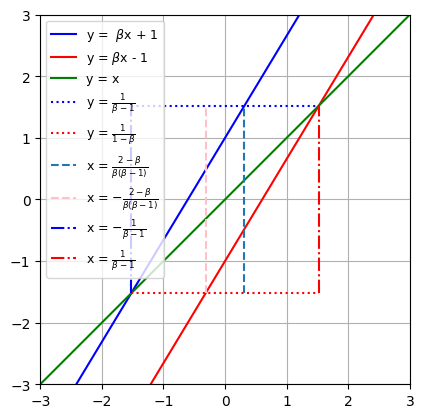
\includegraphics[scale=0.5]{Conclusion2.png}
            \caption{图像}
            \label{fig:C1onclusion2}
      \end{figure*}

      由图像可以看出,当$x\in(-\frac{1}{\beta-1},\frac{2-\beta}{\beta(\beta-1)})$,有$f_1(x)\in(-\frac{1}{\beta-1},\frac{1}{\beta-1})$,而当$x\in(-\frac{2-\beta}{\beta(\beta-1)},\frac{1}{\beta-1})$,有$f_{-1}(x)\in(-\frac{1}{\beta-1},\frac{1}{\beta-1})$。

      而我们又有$(-\frac{1}{\beta-1},\frac{2-\beta}{\beta(\beta-1)})\cup(-\frac{2-\beta}{\beta(\beta-1)},\frac{1}{\beta-1})=(-\frac{1}{\beta-1},\frac{1}{\beta-1})$,故可得,
      $$
            \forall x\in(-\frac{1}{\beta-1},\frac{1}{\beta-1}), \exists i\in\{-1,1\},\mbox{ 使得},f_i(x)\in(-\frac{1}{\beta-1},\frac{1}{\beta-1}).
      $$

      由此,因为$f_{\epsilon_k}(0)=1\in(-\frac{1}{\beta-1},\frac{1}{\beta-1})$,故有,存在一个序列$\{\epsilon_n\}_{n=0}^{k}\in\{-1,1\}$,使得,
      $$
            |\sum_{n=0}^k\epsilon_n\beta^n|<\frac{1}{\beta-1}.
      $$
\end{proof}

\begin{lemma}
      假设$T(x)=F(x)+G(x)$,若有$F:[0,1]\rightarrow\mathbb{R}$是Lipschtz连续的,其Lipschtz常数为$M>0$,$G:[0,1]\rightarrow\mathbb{R}$是连续函数,若$0<r<R<1$且$\frac{R}{r}\in\mathbb{Z}$,则我们有以下不等式:
      $$
                  \underset{a\in[0,1]\times\mathbb{R}}{\sup} N(S(a,\frac{R}{2})\cap\Gamma_T,r)
                  \ge\frac{1}{M+2} \underset{a\in[0.1]\times\mathbb{R}}{\sup}N(S(a,\frac{R}{2})\cap\Gamma_G,r)-\frac{M+2}{\lfloor M\rfloor+2}\frac{R}{r}.
      $$
\end{lemma}

其详细证明可查看[1,第六节]。

\begin{lemma}
      假设$T_{a,b}(x):\mathbb{R}\rightarrow\mathbb{R}$为以下形式的函数:
      $$
            T_{a,b}(x)=\sum_{n=0}^\infty a^nT(b^nx),
      $$
      其中,$T(x):\mathbb{R}\rightarrow\mathbb{R}$是周期为1的$\mathcal{C}^1$连续函数,且$a>0,b>0,ab>1$。若以下两个条件成立:
      \begin{enumerate}
          \item 存在一个常数$C_1>0$,使得,对任意的正整数$M>0$,存在一个正整数$k$使得$J_k=(\frac{k}{b^{M+1}},\frac{k+1}{b^{M+1}})$,且$\forall x_1,x_2\in J_k$,以下不等式成立
          $$
                |\sum_{n=0}^Ma^nT(b^nx_1)-\sum_{n=0}^Ma^nT(b^nx_2)|<C_1|x_1-x_2|.
          $$
          \item 存在一个水平集$L\subset[0,1]$,其下盒维数不小于$D$,即
          $$
                \exists y\in\mathbb{R},\underline{\mathrm{\dim_B}}L(y)=\underline{\mathrm{\dim_B}}\{x\in[0,1]:T_{a,b}(x)=y\}\ge D。
          $$
      \end{enumerate}
      则有以下结论
      $$
        \mathrm{\dim_A\Gamma_{T_{a,b}(x)}}\ge D+1.
      $$
\end{lemma}

上述结论的证明请参见[1,第六节]。

假设$H_{a,b}(x)=\sum_{n=0}^\infty a^nh(b^nx)$,其中$h(x)$为可分割折线函数,
$\mathbb{I}=\{I_1,I_2,\cdots,I_N\}$为$h(x)$在$[0,1]$区间上按$h(x)$的不可导点分割产生的区间族,
其中$I_1,\cdots,I_N$从左到右排列。

$I_J^*$为$h(x)$在$[0,1]$区间上的导数不为$0$的区间长度最大的区间,其上$h(x)$的导数为$K_{J^*}$。

假设$0<a<1,b>1,1<ab<2,n(\mathbb{I})|b$,且$ab$为$k-1$阶Littlewood多项式的根,则我们可得以下结论:

$$
      \mathrm{\dim_A\Gamma_{H_{a,b}(x)}}\ge1+\frac{1}{k}\Big(1+\log_b2|I_J|\Big).
$$

\begin{proof}

    先证明$H_{a,b}(x)$满足引理3中的第一个条件,即,

    若$a,b$满足,$0<a<1,b\ge2,n(\mathbb{I})|b,1<ab<2$,则有 $\exists C_1>0$,
    $\forall M>0,\exists k\in\mathbb{Z}^+$,使得$\forall x_1,x_2\in [\frac{k}{b^M},\frac{k+1}{b^M}]$,有

    $$
    |\sum_{n=0}^Ma^nh(b^nx_1)-\sum_{n=0}^Ma^nh(b^nx_2)|<C_1|x_1-x_2|.
    $$

    对任意的整数$M>0$,我们考虑第$M$级区间,并记其中第$k+1$个区间为

    $$
    I_M(k)=\big[\frac{k}{2b^M},\frac{k+1}{2b^M}\big],k\in\mathbb{Z}.
    $$

    由于我们取的$b$一定为整数,$I_M(k)$可被分为$b$个区间,因此,我们有以下结论

    $$
    h'(b^Mx)=\begin{cases}
        K_{J^*},~~x\in I_M(k),k (\mathrm{mod}b) \in {[}\frac{b}{n(\mathbb{I})}\sum_{i=0}^{J^*-1}n(I_i),\frac{b}{n(\mathbb{I})}\sum_{i=0}^{J^*}n(I_i){)},\\
        -K_{J^*},~~x\in I_M(k),k(\mathrm{mod}b) \in {[}\frac{b}{n(\mathbb{I})}\sum_{i=0}^{N-J^*}n(I_i),\frac{b}{n(\mathbb{I})}\sum_{i=0}^{N+1-J^*}n(I_i){)}.
    \end{cases}
    $$

    我们记$\epsilon_n=\frac{1}{K_{J^*}}h'(b^nx),n=0,1,\cdots,M$。

    因此,$\forall M>0$我们可以找到一列区间$I_M(k_M)\subset I_{M-1}(k_{M-1})\subset\cdots\subset I_1(k_1)$,使得

    $$
    D_M(x)=\sum_{n=0}^Ma^n(h(b^nx))'=\sum_{n=0}^M(ab)^nh'(b^nx)=K_{J^*}\sum_{n=0}^M\epsilon_n(ab)^n.
    $$

    由引理1可知,$D_M(x)$有界,故$\forall M>0,\exists k\in\mathbb{Z}^+$,使得$\forall x_1,x_2\in [\frac{k}{b^M},\frac{k+1}{b^M}]$,有

    $$
    |\sum_{n=0}^Ma^nh(b^nx_1)-\sum_{n=0}^Ma^nh(b^nx_2)|<C_1|x_1-x_2|.
    $$

    由结论4.1,$H_{a,b}(x)$存在一个水平集$L$,其Hausdorff维数不小于$\frac{1}{k}\Big(1+\log_b\2|I_{J^*}|\Big)$,故有$\mathrm{\dim_B}L\ge\mathrm{\dim_H}L\ge\frac{1}{k}\Big(1+\log_b\2|I_{J^*}|\Big)$。

    由此,$H_a,b(x)$满足引理3中的两个条件,故有
    $$
        \mathrm{\dim_A\Gamma_{H_{a,b}(x)}}\ge1+\frac{1}{k}\big(1+\log_b2|I_{J^*}|\big).
    $$
\end{proof}
